\documentclass{article}
\usepackage{amsmath,amsthm}
\usepackage{amssymb,latexsym}
\usepackage{epsfig}
\usepackage{hyperref}
\usepackage{float}
\usepackage{fullpage}
\usepackage{enumerate}
\usepackage{paralist}
\usepackage{graphicx}


\usepackage{tikz}
\usepackage{tikz-dimline}
\usetikzlibrary{calc,patterns,angles,quotes}
\pgfplotsset{compat=1.18}

\newtheorem{theorem}{Theorem}
\newtheorem{corollary}[theorem]{Corollary}
\newtheorem{lemma}[theorem]{Lemma}
\newtheorem{observation}[theorem]{Observation}
\newtheorem{proposition}[theorem]{Proposition}
\newtheorem{definition}[theorem]{Definition}
\newtheorem{claim}[theorem]{Claim}
\newtheorem{fact}[theorem]{Fact}
\newtheorem{assumption}[theorem]{Assumption}
\newtheorem{example}[theorem]{Example}
\newtheorem{conjecture}[theorem]{Conjecture}
\newtheorem{alg}[theorem]{Algorithm}
\newtheorem{protocol}[theorem]{Protocol}
\newtheorem{problem}[theorem]{Problem}

\newcommand{\ip}[2]{\left\langle #1 , #2\right\rangle}
\newcommand{\tr}{\trace}
\newcommand{\setft}[1]{\mathrm{#1}}
\newcommand{\lin}[1]{\setft{L}\left(#1\right)}
\newcommand{\density}[1]{\setft{D}\left(#1\right)}
\newcommand{\unitary}[1]{\setft{U}\left(#1\right)}
\newcommand{\herm}[1]{\setft{Herm}\left(#1\right)}
\newcommand{\pos}[1]{\setft{Pos}\left(#1\right)}
\newcommand{\sep}[1]{\setft{Sep}\left(#1\right)}
\newcommand{\rank}[1]{\operatorname{rank}(#1)}
\newcommand{\ex}{\paragraph{Exercise.}}

\def\I{I}
\def\({\left(}
\def\){\right)}
\def\X{\mathcal{X}}
\def\Y{\mathcal{Y}}
\def\Z{\mathcal{Z}}
\def\W{\mathcal{W}}
\def\yes{\text{yes}}
\def\no{\text{no}}
\def\blog{\textup{log}}
\newcommand{\A}{\spa{A}}
\newcommand{\B}{\spa{B}}
\newcommand{\UA}{U_A}


\newcommand{\myparagraph}[1]{\paragraph{#1.}}

\newcommand{\eps}{\varepsilon}
\newcommand{\epssdp}{\varepsilon_{\rm sdp}}
\newcommand{\bra}[1]{\langle #1|}
\newcommand{\ket}[1]{|#1\rangle}
\newcommand{\braket}[2]{\langle #1|#2\rangle}
\newcommand{\ketbra}[2]{\ket{#1}{\bra{#2}}}
\newcommand{\lmin}[1] {\lambda_{\operatorname{min}}(#1)}
\newcommand{\lmax}[1] {\lambda_{\operatorname{max}}(#1)}
\newcommand{\lhyes} {\operatorname{LH_{yes}}}
\newcommand{\lhno} {\operatorname{LH_{no}}}
\newcommand{\CQ}{\mathcal{CQ}}
\newcommand{\lh}{\operatorname{LH}}
\newcommand{\flh}{\operatorname{5-LH}}
\newcommand{\klhh}{\operatorname{k-LH}}
\newcommand{\qma}{\operatorname{QMA}}
\newcommand{\enc}[1]{\left<#1\right>}

\newcommand{\C}{C}
\newcommand{\Id}{Id} %CHECK
\newcommand{\Exs}[2]{E_{#1}[#2]} %CHECK

\newcommand{\beq}{\begin{equation}}
\newcommand{\eeq}{\end{equation}}

\newcommand{\trace}{{\rm Tr}}

%\newcommand{\dim}{\operatorname{dim}}
\newcommand{\norm}[1]{\left\|\,#1\,\right\|}       % norm
\newcommand{\pnorm}[1]{\left\|\,#1\,\right\|_p}       % norm
\newcommand{\onorm}[1]{\norm{#1}_{\mathrm{1}}}      % Euclidean norm for vectors
\newcommand{\enorm}[1]{\norm{#1}_{\mathrm{2}}}      % Euclidean norm for vectors
\newcommand{\trnorm}[1]{\norm{#1}_{\mathrm {tr}}}  % trace norm
\newcommand{\fnorm}[1]{\norm{#1}_{\mathrm {F}}}    % frobenius norm
\newcommand{\snorm}[1]{\norm{#1}_{\mathrm {\infty}}}    % spectral norm

\newcommand{\set}[1]{{\left\{#1\right\}}}    % braces for set notation
\newcommand{\ve}[1]{\mathbf{#1}}
\newcommand{\abs}[1]{\left\lvert #1 \right\rvert}
\newcommand{\optprod}{\OPT_P}
\newcommand{\opt}{\operatorname{OPT_1}}
\newcommand{\optt}{\operatorname{OPT_2}}
\newcommand{\newopt}{\operatorname{NEW-OPT}}
\newcommand{\swap}{\operatorname{SWAP}}
\newcommand{\poly}{\operatorname{poly}}
\newcommand{\cc}{d^{\frac{k}{2}}}
\newcommand{\OPT}{{\rm OPT}}
\newcommand{\QMA}{{\rm QMA}}
\newcommand{\MQA}{{\rm MQA}}
\newcommand{\NP}{{\rm NP}}
\newcommand{\PP}{{\rm P}}
\newcommand{\PH}{{\rm PH}}
\newcommand{\BPP}{{\rm BPP}}
\newcommand{\BQP}{{\rm BQP}}
\newcommand{\TCSP}{{\rm 2-CSP}}

\newcommand{\complex}{{\mathbb C}}
\newcommand{\reals}{{\mathbb R}}
\newcommand{\ints}{{\mathbb Z}}
\newcommand{\nats}{{\mathbb N}}

\newcommand{\spa}[1]{\mathcal{#1}}
\newcommand{\dens}{\mathcal{D}(\spa{A}\otimes\spa{B})}
%\newcommand{\unitaries}{U(\spa{A}\otimes\spa{B})}

\newcommand{\LL}{\mathcal{L}}
\newcommand{\DD}{\mathcal{D}}
\newcommand{\HH}{\mathcal{H}}
\newcommand{\UU}{\mathcal{U}}

\mathchardef\mhyphen="2D

\newcommand{\ayes}{A_{\rm yes}} %CHECK
\newcommand{\ano}{A_{\rm no}} %CHECK
\newcommand{\nl} {\mathcal{L}_1}

\bibliographystyle{alpha}

\begin{document}

\title{\vspace{-10mm}Introduction to Quantum Computation, UPB\\Winter 2022, Assignment 1\\{\large To be completed by: Friday, October 21}}
\date{}
\maketitle

\section{Exercises}
\begin{enumerate}
  \item %($5$ marks)
        For complex number $c=a+bi$, recall that the \emph{real} and \emph{imaginary} parts of $c$ are denoted $\operatorname{Re}(c)=a$ and $\operatorname{Imag}(c)=b$.
        \begin{enumerate}
          \item %($1$ mark)
                Prove that $c+c^\ast=2\cdot \operatorname{Re}(c)$.

                \begin{proof}
                  \begin{equation}
                    c+c^\ast = (a+bi) + (a-bi) \overset{\text{assoc., comm.}}{=}
                    (a + a) + (b - b)i = 2a = 2Re(c)
                  \end{equation}
                \end{proof}
          \item %($2$ marks)
                Prove that $cc^\ast={a}^2+{b}^2$. How can we therefore rewrite $\abs{c}$ in terms of $a$ and $b$?

                \begin{proof}
                  \begin{equation}
                    cc^\ast=(a+bi)(a-bi)=a^2-(bi)^2=a^2-i^2b^2=a^2-(-1)b^2=a^2+b^2
                  \end{equation}
                \end{proof}
          \item %($1$ mark)
                What is the polar form of $c=\frac{1}{\sqrt{2}}+\frac{1}{\sqrt{2}}i$? Use the fact that $e^{i\theta}=\cos\theta+i\sin\theta$.
                \begin{observation}
                  $$c=1\cdot e^{\frac{\pi}{4}i}\overset{\text{by calculation}}{=}c$$
                  Where:\\
                  Length: $1$\\
                  Angle: $\frac{\pi}{4}$
                \end{observation}

          \item %($1$ mark)
                Draw $c=\frac{1}{\sqrt{2}}+\frac{1}{\sqrt{2}}i$ as a vector in the complex plane, ensuring to denote both the length of the vector and its angle with the $x$ axis.

                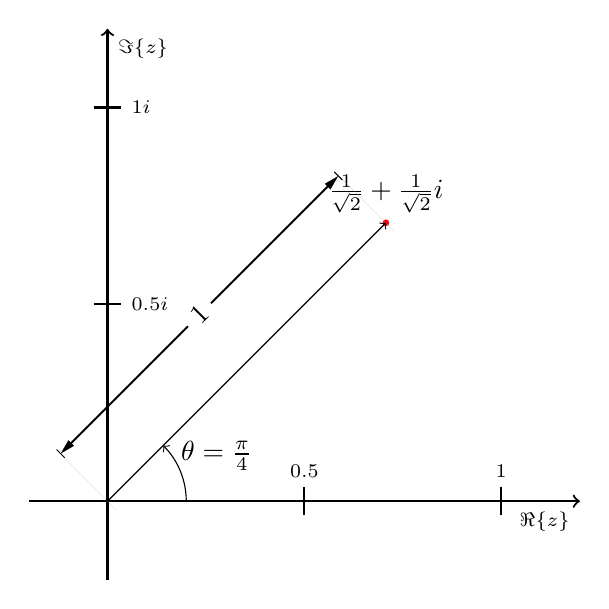
\begin{tikzpicture}[scale=5]
                  \begin{scope}[thick,font=\scriptsize]
                    % Axes:
                    % Are simply drawn using line with the `->` option to make them arrows:
                    % The main labels of the axes can be places using `node`s:
                    \draw [->] (-0.2,0) -- (1.2,0) node [below left]  {$\Re\{z\}$};
                    \draw [->] (0,-0.2) -- (0,1.2) node [below right] {$\Im\{z\}$};

                    % Axes labels:
                    % Are drawn using small lines and labeled with `node`s. The placement can be set using options
                    \iffalse% Single
                      % If you only want a single label per axis side:
                      \draw (1,-3pt) -- (1,3pt)   node [above] {$1$};
                      \draw (-1,-3pt) -- (-1,3pt) node [above] {$-1$};
                      \draw (-3pt,1) -- (3pt,1)   node [right] {$i$};
                      \draw (-3pt,-1) -- (3pt,-1) node [right] {$-i$};
                    \else% Multiple
                      % If you want labels at every unit step:
                      \foreach \n in {0.5,1}{%
                          \draw (\n,-1pt) -- (\n,1pt)   node [above] {$\n$};
                          \draw (-1pt,\n) -- (1pt,\n)   node [right] {$\n i$};
                        }
                    \fi
                  \end{scope}
                  % Vector:
                  % Draw the point with a filled in circle:
                  \draw[red,fill=red] ({1/sqrt(2)},{1/sqrt(2)}) circle (0.2pt);
                  % Is drawn using a line with the `->` option:
                  \draw [->] (0,0) -- ({1/sqrt(2)},{1/sqrt(2)}) node [above] {$\frac{1}{\sqrt{2}}+\frac{1}{\sqrt{2}}i$};
                  % draw the angle
                  \coordinate (x) at (1,0);
                  \coordinate (origin) at (0,0);
                  \coordinate (point) at ({1/sqrt(2)},{1/sqrt(2)});
                  \draw pic[draw, ->, "$\theta=\frac{\pi}{4}$", angle radius=1cm, angle eccentricity=1.5] {angle = x--origin--point};
                  % draw the length as a dimline
                  \dimline[line style = {line width=0.7pt},
                    extension start length=0.2,
                    extension end length=0.2] {($ (origin) + (-0.12,0.12) $)} {($ (point) + (-0.12,0.12) $)} {$1$};
                \end{tikzpicture}
        \end{enumerate}
  \item %($4$ marks)
        Prove that for any normalized vectors $\ket{\psi},\ket{\phi}\in\complex^d$,
        \[
          \enorm{\ket{\psi}-\ket{\phi}}=\sqrt{2-2\cdot\operatorname{Re}(\braket{\psi}{\phi})}.
        \]
        \begin{proof}
          \begin{equation}
            \begin{aligned}
              \enorm{\ket{\psi}-\ket{\phi}} & =\sqrt{\braket{\psi-\phi}{\psi-\phi}}                                                                          \\
                                            & =\sqrt{\braket{\psi}{\psi}-\braket{\psi}{\phi}-\braket{\phi}{\psi}+\braket{\phi}{\phi}}                        \\
                                            & =\sqrt{1-\braket{\psi}{\phi}-\braket{\phi}{\psi}+1}=\sqrt{2-\braket{\psi}{\phi}-\braket{\psi}{\phi}^\ast}      \\
                                            & =\sqrt{2-(\braket{\psi}{\phi}+\braket{\psi}{\phi}^\ast)}=\sqrt{2-2\cdot\operatorname{Re}(\braket{\psi}{\phi})} \\
            \end{aligned}
          \end{equation}
        \end{proof}
        Why does it not matter if we replace $\braket{\psi}{\phi}$ with $\braket{\phi}{\psi}$ in this equation?

        It does not matter, since $\braket{\psi}{\phi}=\braket{\phi}{\psi}^\ast$, and this implies that $\operatorname{Re}(\braket{\psi}{\phi})=\operatorname{Re}(\braket{\phi}{\psi})$.
  \item %($6$ marks)
        Define
        \[
          A=\left(
          \begin{array}{cc}
              a & b \\
              c & d \\
            \end{array}
          \right).
        \]
        \begin{enumerate}
          \item %($2$ marks)
                What is $\trace(A\cdot \ketbra{1}{0})$? (Hint: This can be computed quickly by using the cyclic property of the trace and the outer product representation of $A$. Do master this trick; it will be used repeatedly in the course and save you much time.)

                \begin{equation}
                  \trace(A\cdot \ketbra{1}{0})=\trace(\bra{0}A\ket{1})=A_{0,1}=b.
                \end{equation}
          \item %($4$ marks)
                Let $\ket{+}=\frac{1}{\sqrt{2}}(\ket{0}+\ket{1})$. Use the same tricks as in part $A$, along with the fact that the trace is linear, to quickly evaluate
                \[
                  \trace(A\cdot\ketbra{+}{+}).
                \]

                \begin{equation}
                  \begin{aligned}
                    \trace(A\cdot\ketbra{+}{+}) & =                                        & \trace & (\bra{+}A\ket{+})                                                 & \\
                                                & = \left(\frac{1}{\sqrt{2}}\right)^2\cdot & \trace & ((\bra{0}+\bra{1})A(\ket{0}+\ket{1}))                             & \\
                                                & = \frac12\cdot                           & \trace & (\bra{0}A\ket{0}+\bra{0}A\ket{1}+\bra{1}A\ket{0}+\bra{1}A\ket{1}) & \\
                                                & = \frac12\cdot                           &        & (a+c+d+b)
                  \end{aligned}
                \end{equation}
        \end{enumerate}
  \item %($5$ marks)
        \begin{enumerate}
          \item %($2$ marks)
                A general property of the outer product is that $(\ketbra{\psi}{\phi})^\dagger=\ketbra{\phi}{\psi}$. Verify that this holds for the case where $\ket{\psi}=\ket{0}$ and $\ket{\phi}=\ket{1}$. (Hint: Write out the full matrix corresponding to $\ketbra{0}{1}$.)

                \begin{equation}
                  \begin{aligned}
                    \ketbra{0}{1} = \left(
                    \begin{array}{cc}
                        0 & 1 \\
                        0 & 0 \\
                      \end{array}
                    \right) \\
                    (\ketbra{0}{1})^\dagger = \left(
                    \begin{array}{cc}
                        0 & 0 \\
                        1 & 0 \\
                      \end{array}
                    \right) = \ketbra{1}{0}
                  \end{aligned}
                \end{equation}
          \item %($3$ marks)
                Use Part (a) to prove that a normal matrix $A$ satisfies $A=A^\dagger$ if and only if all of $A$'s eigenvalues are real. (Hint: Since $A$ is normal, you can start by writing $A$ in terms of its spectral decomposition. What does the condition $A=A^\dagger$ enforce in terms of $A$'s spectral decomposition?)

                Let $$A = \sum_{i=1}^d \lambda_i \ketbra{\psi_i}{\psi_i}$$ be the spectral decomposition of $A$.
                Where $\lambda_i$ are the eigenvalues of $A$ and $\ket{\psi_i}$ are the corresponding eigenvectors
                such that the set of eigenvectors form an orthonormal basis of $\complex^d$.

                Direction $\Rightarrow$: $A$ satisfies $A=A^\dagger$. We show that all eigenvalues are real.
                \begin{proof}
                  Since $A=A^\dagger$, we have:
                  \begin{equation}
                    \begin{aligned}
                      A=\sum_{i=1}^d \lambda_i \ketbra{\psi_i}{\psi_i}=\left(\sum_{i=1}^d \lambda_i \ketbra{\psi_i}{\psi_i}\right)^\dagger=A^\dagger
                    \end{aligned}
                  \end{equation}
                  \begin{equation}
                    \begin{aligned}
                      \left(\sum_{i=1}^d \lambda_i \ketbra{\psi_i}{\psi_i}\right)^\dagger & =\sum_{i=1}^d \left(\lambda_j \ketbra{\psi_i}{\psi_i}\right)^\dagger \\
                                                                                          & =\sum_{i=1}^d \lambda_j^\dagger (\ketbra{\psi_i}{\psi_i})^\dagger    \\
                                                                                          & =\sum_{i=1}^d \lambda_j^\dagger \ketbra{\psi_i}{\psi_i}
                    \end{aligned}
                  \end{equation}
                  All $\ketbra{\psi_i}{\psi_i}$ are linearly independent, which can be easily seen by writing them out in the basis
                  of $\ket{\psi_i}$.

                  Now:
                  \begin{equation}
                    \begin{aligned}
                      \sum_{i=1}^d \lambda_i \ketbra{\psi_i}{\psi_i}=\sum_{i=1}^d \lambda_j^\dagger \ketbra{\psi_i}{\psi_i}
                    \end{aligned}
                  \end{equation}

                  Which means that
                  \begin{equation}
                    \lambda_i=\lambda_i^\dagger \quad \forall i
                  \end{equation}

                  From which it follows, that all eigenvalues are real.
                \end{proof}

                Direction $\Leftarrow$: All eigenvalues are real. We show that $A=A^\dagger$.

                \begin{proof}
                  Since
                  \begin{equation}
                    \lambda_i=\lambda_i^\dagger \quad \forall i
                  \end{equation}

                  It follows that:
                  \begin{equation}
                    \begin{aligned}
                      \sum_{i=1}^d \lambda_i \ketbra{\psi_i}{\psi_i}=\sum_{i=1}^d \lambda_j^\dagger \ketbra{\psi_i}{\psi_i}
                    \end{aligned}
                  \end{equation}

                  By the same argument as above:
                  $$A=A^\dagger$$
                \end{proof}
        \end{enumerate}

\end{enumerate}

\end{document}
